\documentclass{PHlab-thesis}
\usepackage{graphicx}

\addbibresource{thesis.bib}

\newcommand*\Department中文{資訊工程學研究所}
\newcommand*\Department英文{Institute of Computer Science and Information Engineering}

\newcommand*\ThesisTitle中文{亞硫酸氫鹽測序數據的甲基化調用軟體之基準評估\退{1}}
\newcommand*\ThesisTitle英文{Benchmark evaluation of methylation calling software for bisulfite sequencing data}
% \newcommand*\ThesisNote中文{示例:其實徐翡曼是東京大學畢業的博士}% For real thesis omit, or use {初稿} etc.
% \newcommand*\ThesisNote英文{Just an example.  Fei-Man actually graduated from Tokyo Univ.}% For real thesis omit, or use {draft} etc.

\newcommand*\Student中文{許芊瑀}
\newcommand*\Student英文{Chien-yu Hsu}

\newcommand*\Advisor中文{賀保羅}
\newcommand*\Advisor英文{Paul Horton}

%% 果有共同指導老師可以用:
%% \newcommand*\CoAdvisorA中文{}
%% \newcommand*\CoAdvisorA英文{}
%% \newcommand*\CoAdvisorB中文{}
%% \newcommand*\CoAdvisorB英文{}


\newcommand*\YearMonth英文{July, 2022}
\newcommand*\YearMonth中文{111年7月}

\pagestyle{fancy}% Use fancyhdr
\begin{document}


\newcommand*\Keywords英文{DNA methylation, bisulfite sequence, methylation calling tools}
\newcommand*\Abstract英文{%
DNA methylation is one of the important epigenetic mechanisms and that are also involved in many biological processes, including transcriptional activity, genomic imprinting, development, and many diseases including cancer. In recent years, advances in next-generation sequencing technologies have provided opportunities to study genome-wide DNA methylation\cite{sun2018comprehensive}. In addition, bisulfite sequencing is now a popular and powerful method for methylation detection and is also the most studied method. Whole gene bisulfite sequencing (WGBS) and reduced representation bisulfite sequencing (RRBS) are often used to generate DNA methylation ,and efficient tools are needed to compare bisulfite sequencing data\cite{medvedeva2014effects}.

In this paper, we will analyze three methylation calling tools: EAGLE-METH, BS-Seeker2 and Bismark, to compare their ability to assess the methylation-level and discuss the impact on the analysis of the methylation-level in data of different species or from different chromosomal fragments.
}


\newcommand*\Keywords中文{DNA甲基化、亞硫酸氫鹽測序、對齊工具}
\newcommand*\Abstract中文{%
DNA甲基化是重要的表觀遺傳機制之一,DNA甲基化也涉及許多生物學過程,包括轉錄活性、基因組印記、發育和包括癌症在內的許多疾病。近幾年,隨著新一代測序技術的進步,為研究全基因組DNA甲基化提供了機會\cite{sun2018comprehensive}。另外,亞硫酸氫鹽測序為現在流行且強大的甲基化檢測方法,同時也是最多人研究的方法。全基因亞硫酸氫鹽測序(WGBS)和還原型亞硫酸氫鹽測序(RRBS)經常被用於生成DNA甲基化組,需要高效的工具來比對亞硫酸氫鹽測序數據\cite{medvedeva2014effects}。

我們將在此篇論文分析EAGLE-METH、BS-Seeker2和Bismark這三種對齊工具,比較其評估甲基化程度的能力,並討論在不同物種的數據或是不同染色體片段中,對於分析甲基化水平的影響。
}

\newcommand*\Acknowledgements{%
感謝我...}



\newcommand*\SelectFontsize[2]{\fontsize{#1}{#1}\selectfont\mdseries#2\par}
\newcommand*\SelectFontsizeBF[2]{\fontsize{#1}{#1}\selectfont\bfseries#2\par}
\newcommand*\SignatureRule[1][6]{\rule{#1cm}{0.3mm}}
\newcommand*\AddToContents[1]{\newpage\phantomsection\addcontentsline{toc}{chapter}{#1}}

\doublespace
\pagenumbering{gobble}
\renewcommand{\thefootnote}{\fnsymbol{footnote}}


\begin{center}
\vspace{2cm}
\SelectFontsizeBF{24}{%
\University中文\Department中文\\
\學位 論文}

\vfill
\SelectFontsizeBF{24}{\ThesisTitle中文}
\ifdefined\ThesisNote中文
\SelectFontsize{22}{\textit{\ThesisNote中文}}
\fi

\vspace{5mm}
\SelectFontsizeBF{22}{\ThesisTitle英文}
\ifdefined\ThesisNote英文
\SelectFontsize{20}{\textit{\ThesisNote英文}}
\fi

\vfill

\begin{minipage}{\linewidth}
{\setlength\tabcolsep{0pt}
%
\begin{tabular}{ Wr{5em} Wl{6em} Wr{5em} wl{7em} }
研究生:   & ~~\Student中文  &      Student: & ~~\Student英文\\
指導老師: & ~~\Advisor中文  &      Advisor: & ~~\Advisor英文\\
\ifdefined\CoAdvisorA中文
共同指導: & ~~\CoAdvisorA中文 &   Co-Advisor: & ~~\CoAdvisorA英文\\
\fi
\ifdefined\CoAdvisorB中文
         & ~~\CoAdvisorB中文 &   Co-Advisor: & ~~\CoAdvisorB英文\\
\fi
\end{tabular}
}
\end{minipage}

\vfill
\SelectFontsize{18}{%
National Cheng Kung University,\\
Tainan, Taiwan, R.O.C.\\
Thesis for \ifdef\PhD{Doctor of Philosophy}{Master of Science} Degree\\
\YearMonth英文}

\vfill
\SelectFontsize{20}{中華民國\YearMonth中文}
\end{center}



\ifdefined\optCommittee
\newpage
\begin{center}
\vspace{1cm}
\SelectFontsizeBF{24}{%
\University中文\Department中文\\
\學位 論文}
\vfill
\SelectFontsizeBF{20}{\ThesisTitle中文}
\end{center}

\vfill
\SelectFontsize{20}{%
\noindent 研究生:\Student中文\\
本論文業經審查及口試合格特此證明}


\begin{center}
\SelectFontsize{18pt}{論文考試委員}
\vfill
\SignatureRule \hspace*{1cm} \SignatureRule
\vfill

\SignatureRule \hspace*{1cm} \SignatureRule
\vfill

指導教授:\SignatureRule[8]
\vfill
  所長:\SignatureRule[8]

\vfill
\SelectFontsize{18}{中華民國 \hspace{2em} 年 \hspace{2em} 月 \hspace{2em} 日}
\end{center}


\newpage
\begin{center}
\vspace{1cm}
\SelectFontsize{18}{\University英文, \Department英文}
\SelectFontsize{19}{\ifdef\PhD{Ph.D.}{Master's} Degree Thesis}

\vfill
\SelectFontsizeBF{20}{\ThesisTitle英文}
\end{center}

\vfill
\SelectFontsize{18}{Student: \Student英文}

\SelectFontsize{18}{%
A thesis submitted to the graduate division in partial fulfillment of the requirement for the degree of
\ifdef\PhD{Doctor of \mbox{Philosophy}}{Master of Science}.
}

\vfill
\begin{center}
\SelectFontsize{18}{Approved by}

\vfill
\SignatureRule \hspace*{1cm} \SignatureRule

\vfill
\SignatureRule \hspace*{1cm} \SignatureRule

\vfill
Advisor: \SignatureRule[8]

\vfill
Chairman: \SignatureRule[8]

\vfill
\SelectFontsize{18}{\YearMonth英文}
\vspace*{20pt}
\end{center}
\fi% optCommittee


\AddToContents{中文摘要}
\setcounter{page}{1}
\pagenumbering{roman}


\begin{center}
\SelectFontsizeBF{24}{\ThesisTitle中文}

\vspace{4mm}
\SelectFontsize{18}{\Student中文\footnote[1]{學生} ~ \Advisor中文\footnote[2]{指導教授}}

\vspace{5mm}
\SelectFontsize{20}{國立成功大學\Department中文}

\vspace{12mm}
\makebox[2.7cm][c]{\SelectFontsizeBF{22}{摘要}}
\end{center}

\vspace{4mm}
\SelectFontsize{16}{\Abstract中文}

\vspace{4mm}
\begin{flushleft}
\SelectFontsize{16}{\textbf{關鍵詞:} \Keywords中文}
\end{flushleft}



\AddToContents{Abstract}
\begin{center}
\SelectFontsizeBF{22}{\ThesisTitle英文}

\vspace{4mm}
\SelectFontsize{18}{\Student英文\footnote[1]{Student} ~ \Advisor英文\footnote[2]{Advisor}}

\vspace{4mm}
\SelectFontsize{16}{\Department英文, National Cheng Kung University}

\vspace{12mm}
\SelectFontsizeBF{20}{Abstract}
\end{center}

\vspace{4mm}
\SelectFontsize{14}{\Abstract英文}

\vspace{4mm}
\begin{flushleft}
\SelectFontsize{16}{\textbf{Keywords:} \Keywords英文}
\end{flushleft}



\AddToContents{誌謝}
\begin{center}\SelectFontsizeBF{24}{誌謝}\end{center}

\vspace{4mm}
\Acknowledgements



\renewcommand{\contentsname}{CONTENTS}
\AddToContents{Contents}
\tableofcontents


\AddToContents{List of Tables}
\listoftables


\AddToContents{List of Figures}
\listoffigures
% 封面頁, 口委中英文簽名單, 誌謝, 中英文摘要, 論文目錄, 圖表目錄


%────────────────────  List of Symbols  ────────────────────
\renewcommand\nomgroup[1]{%
  \item[\bfseries
  \ifstrequal{#1}{A}{General}{%
  \ifstrequal{#1}{Z}{Gene/Protein Names}%
  }]}

\nomenclature[A]{$\lg$}{Logarithm base 2}
\nomenclature[A]{KL\ Divergence}{Kullback-Liebler Divergence}
\nomenclature[Z]{Myc}{MYC proto-oncogene}
\nomenclature[Z]{USF-1}{Upstream stimulatory factor 1}

\printnomenclature[5cm]

\newpage
\setcounter{page}{1}
\pagenumbering{arabic}



\chapter{Introduction}
\section{Background}
DNA methylation is a form of chemical modification of DNA that can affect genetic performance without changing the DNA sequence\cite{guo2013bs}. DNA methylation is also one of the important epigenetic mechanisms involved in many fundamental biological processes, such as development, aging, response to environmental changes and response to diet. It may also be disordered in a few human diseases, including cancer, diabetes, Alzheimer’s disease, and Parkinson’s disease, all of which show abnormal DNA methylation. In animals, DNA methylation occurs mainly at the cytosine of the dinucleotide CpG ,and a methyl group is added at its carbon 5 position (Figure \ref{f1}). In humans, 80-90\% of CpG dinucleotides are methylated. Therefore, DNA methylation is now a very important study.

\begin{figure}[h!]
  \centering
  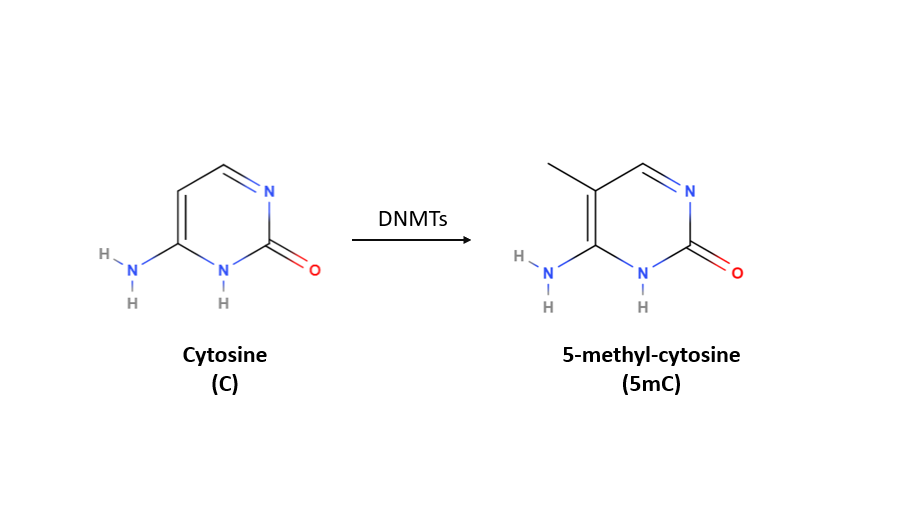
\includegraphics[scale=0.8]{figures/dna_methylation.png}
  \caption{\textbf{A diagram illustrating how DNA methylation works.}
  DNA methylation is the addition of a chemical group -methyl (-CH3) to the carbon atom structure at the 5' end of cytosine on the DNA sequence. DNA methyltransferases (DNMTs) are the write-in proteins for methylation, and DNA methylation is affected by DNA methyltransferases, which are mainly DNMT1, DNMT3A, and DNMT3B. }
  \label{f1}
\end{figure}

Bisulfite sequencing is the most commonly used method to determine DNA methylation today and is considered the gold standard for DNA methylation analysis. Bisulfite sequencing is performed using next-generation sequencers that provide genome-wide measurements of DNA methylation at single-nucleotide resolution. Treatment of DNA with bisulfite converts cytosine residues to uracil; however, the methylated cytosine remains unaffected. Therefore, only the methylated cytosine is retained in the DNA fragments treated with bisulfite. Based on this property, bisulfite can detect the methylation of single nucleotides.

After the above steps, PCR was then used to change the uridine (U) to thymine (T) in the bisulfite DNA sequence. After PCR amplification, we can see that the unmethylated cytosine (C) becomes thymine (T), and the opposite strand corresponds to guanine (A). On the other hand, cytosines that are methylated are not affected.

\section{Motivation}
DNA methylation is a chemical modification and plays an important role in cancer and many complications. Therefore, the study of DNA methylation is very important. The most commonly used gold standard technique to measure DNA methylation today is bisulfite sequencing. The sequence of DNA is altered by bisulfite treatment, and this alteration makes bisulfite sequencing data computationally difficult.

Therefore, in this paper, we analyze bisulfite sequencing data using real and simulated datasets to help us evaluate the performance of different tools. The methylation level of CpG will be the main basis for our evaluation of the accuracy of the tools, which will be calculated based on the number of methylated reads mapped to the reference genome and the number of unmethylated reads. Accurate mapping is also very important here, as it can lead to biased estimates of DNA methylation levels. Therefore, it is very important to evaluate the accuracy of the methylation call of different mapping algorithms.

\section{Research framework}
In the first chapter, we describe the background of DNA methylation and what diseases it will cause in humans, as well as introduce the process of bisulfite sequencing. Our motivation will be to describe the importance of methylation analysis.

In the second chapter, we introduce the simulation tool MethylFASTQ used in the experiment, as well as the three different bisulfite sequencing methylation calling tools and bowtie2.

In the third chapter, the experimental results of real data and simulated data are recorded and comparison of the methylation levels in different comparison tools is shown.

In the fourth chapter, we summarize the results of the previous chapter and discuss the future improvements of EAGLE-meth.


\chapter{Materials and Related works}

\section{MethylFASTQ}
There are many tools available today for analyzing bisulfite data, but the wide range of biology and technical variability of the data makes it difficult to determine which tool to choose for the analysis. We can evaluate the performance of the tools using real and simulated data sets to obtain more accurate analyses. Since bisulfite sequencing experiments are time consuming and costly, using synthetic simulated data is becoming more and more popular. Compared to real data sets created in the laboratory, simulated data sets are relatively fast and inexpensive in terms of both time and experimental cost, and simulated data can quickly generate a large amount of data. In addition, simulated data can be used to evaluate software performance and to explore innovative computational tools.

In this paper, we will use the simulation tool MethylFASTQ\cite{piaggeschi2019methylfastq}, an easy-to-use bioinformatics tool, which is written in Python, starting from a given reference genome, and outputting a synthetic bisulfite dataset in FASTQ format.  The FASTQ file is a text format capable of storing biological data sequenced by NGS, as well as sequencing scores.  The information in the FASTQ file includes the unique id of each read sequence, which provides information about its true mapping position in the reference genome, and the mass score, which is a measure of the mass associated with the base group in the sequence. At the same time, MethylFASTQ also provides a number of parameters that can be adjusted, such as read length, sequencing mode, coverage and number of sequencing errors. The coverage parameter indicates the number of times each base is sequenced or the number of reads aligned to a single base.

First, we choose the human genome as the reference gene, and after MethylFASTQ processing, two types of files are generated:
(i) FASTQ file(s) that contains the sequenced reads.
(ii) methylation call file that contains the true methylation call of each sequenced cytosine.
In the case of single-ended sequencing, a FASTQ file(s) will be generated. In the case of double-ended sequencing, two FASTQ files are generated, considering both forward and reverse reads.

In addition, MethylFASTQ can simulate two types of experiments, whole genome bisulfite sequencing (WGBS) and targeted bisulfite sequencing experiments. In the case of WGBS, a sorted list of chromosome names can be used, while if no list of chromosome names is provided, the entire reference genome will be sequenced. The targeted-BS mode requires a list file of the genomic regions to be sequenced, which includes:
(1) the chromosome ID;
(2) the starting bp of the region to be sequenced; 
(3) the last bp of the region to be sequenced. 
In the next section, we will use the synthesis data generated by MethylFASTQ as input to compare the performance of EAGLE-METH, BS-Seeker2 and Bismark on alignment and methylation calling.

\section{Methylation calling tools}
Currently, the main sequencing libraries for DNA methylation studies include: WGBS (whole genome bisulfite sequencing) and RRBS (Reduced Representation Bisulfite Sequencing). The main tools used for comparing bisulfite sequence data and drawing DNA methylation profiles are: BS-Seeker2, Bismark and BSMAP.  Meth-Eagle modified by EAGLE, and the BS-Seeker2 and Bismark tools will be introduced in the following sections. 

Due to a combination of several factors,the alignment of bisulfite-treated sequences to the reference genome poses significant computational challenges. Such as the reduced complexity of the DNA code and up to four DNA strands to be analyzed, among others. Even though there are many excellent short-read mapping tools available, e.g., Bowtie, it does not have the capability to perform bisulfite mapping by itself. Therefore, two algorithms have been proposed for bisulfite sequencing: wildcard and three-letter, and this paper will focus on the introduction of three-letter aligners\cite{krueger2011bismark}. In addition, the methylation level of CpG sites is calculated based on the number of methylated and unmethylated reads mapped to the reference genome, so the mapping rate of reads is also an important factor affecting the accuracy of methylation evaluation.

In general, in mammals, DNA methylation occurs mainly on CpG dinucleotides. However, in embryonic stem cells, a certain amount of non-CpG methylation is shown. In plants, methylation is common in both symmetrical CpG or CHG and asymmetrical CHH environments (the H mentioned above can be A, T or C). Therefore, in the following alignment tool, we will consider these three methylation scenarios for methylation analysis and evaluation.

\section{EAGLE-meth}
EAGLE-meth is a modified generative probability model based on EAGLE\cite{kuo2018eagle}, which calculates the probability of methylation of the CpG site and gives a likelihood value to the site. EAGLE itself is a method to calculate the probability of genomic variation, which is extended to explore the gene sequence and evaluate the probability of methylation of each cytosine in the sequence.

EAGLE-meth has three main input files, the reference genome, VCF and reads, which are different from the original EAGLE because the reads are bisulfite treated and contain both mutation and methylation information. First, we will use the BWA-meth tool to compare the reads with the reference genome sequence.  BWA-meth is an alignment tool designed to deal with bisulfite sequences, which is similar to BWA-MEM, but the difference is whether the sequences used are bisulfite treated or not.  Second, it converts the generated SAM file to BAM file format, and sorts and indexes the file.  Third, referring to EAGLE's work, we give two different hypothetical sequences, one is a hypothetical reference sequence and the other is a hypothetical alternative sequence. The hypothetical reference sequence assumes that all CpGs in the reference sequence will be methylated, while the hypothetical alternative sequence assumes whether each CpG is methylated or not, and all possible combinations of methylation are considered.  Then, these two sequences were aligned with the reads and their likelihoods were calculated separately.  Fourth, we selected the sequence with higher likelihood and calculated the marginal probability of that sequence. In the subsequent analysis of the tool, we will use the marginal probability as a criteria to evaluate the occurrence of methylation.

\section{BS-Seeker2}
Since conventional aligners are not specifically designed for bisulfite treatment reads, BS-Seeker2 was chosen as the aligner of choice in this case.  BS-Seeker2 is a method that converts a genome into a three-letter alphabet and aligns the bisulfite treatment reads with the reference genome using Bowtie2.

The BS-Seeker2 is a modified version of the BS-Seeker. The actual BS-Seeker2 procedure can be divided into three steps: (1) creating an index for the BS-seq data; the indexes for RRBS and WGBS are created by three letter-transformed genomes respectively; (2) aligning the reads with the indexes; (3) calculating the methylation levels of each base site, and The three output files (wiggle, CGmap, and ATCGmap files) were generated from the BAM/SAM in the previous step. (Figure \ref{f2}) shows the flowchart of BS-Seeker2 considering only the WGBS case\cite{guo2013bs}.

\begin{figure}[h!]
  \centering
  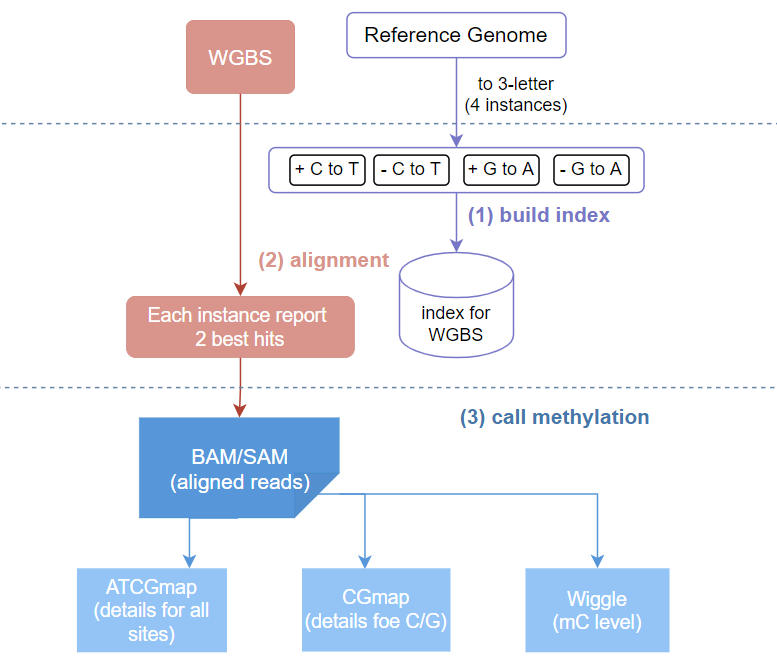
\includegraphics[scale=0.8]{figures/bs_seeker2_workflow.png}
  \caption{\textbf{The main steps in the workflow of BS-Seeker2 in the case of WGBS.}
  The "2 best hits per instance" in step 2 means 2 instances for directional,4 for un-directional.}
  \label{f2}
\end{figure}

Furthermore, BS-Seeker2 supports a variety of library types, including WGBS and RRBS, single-end or paired-end sequencing, and directional or non-directional libraries. The supported input file formats are fasta, fastq, qseq, and pure sequence (one-line one-sequence). The supported alignment tools are bowtie2, bowtie, SOAP, which can be used to support local alignment and gap alignment. Using different alignment tools, BS-Seeker2 will generate different indexes. BS-Seeker2 has designed different index building strategies for WGBS and RRBS, and the indexes built by BS-Seeker2 in RRBS are smaller than those built in WGBS. Through reducing the indexes, the search space for sequence alignment is significantly reduced, thus improving the computational efficiency and mapping accuracy. For example, creating indexes for the human genome is a time-consuming task. Due to the huge amount of data in the human genome, this step can take several hours.

After creating the index, we can proceed to the sequence alignment step.  The formats of input files supported include BAM, SAM, and BS-seeker. BS-Seeker2 can automatically identify the file format by the input files. By doing this, large data can be divided into smaller pieces and run simultaneously, so it is also the easiest step to reduce time and increase efficiency. In addition, although BS-Seeker2 like the other software, also provides a paired-end alignment mode. But in fact, in the alignment procedure, using single-ended mode can be more accurate and efficient than pair-ended mode.  For the pair-ended mode of bisulfite data,It is recommended to use the single-ended mode for each mate and then merge all the generated BAM files together.

The last step is calculating the methylation level of each base site. At the same time, it can be decided in this step whether to filter the not converted reads or not. Because some reads are extremely amplified during PCR, this step helps us to obtain unique reads before mapping. When calculating methylation levels, this step can take longer, around ten hours, if the data are whole genome bisulfite sequenced (WGBS) or modified bisulfite linked markers (PBRT) and the genome is large, such as human and mouse. In this step, BS-Seeker2 reads in the bam files and then sorts the bam files and creates a bai file index. If the files are already sorted, you can set the parameter “–sorted” to False to save the calculation time. There are three output files, wig file, CGmap file and ATCGmap file, and the main information recorded includes chromosome, forward and reverse strand information, position and methylation-level, etc.

\section{Bismark}
The combination of DNA bisulfite processing and high-throughput sequencing captures the state of the cellular epigenome by revealing genome-wide cytosine methylation at single-base resolution.  Bismark is a flexible tool for analyzing bisulfite sequence data, and Bismark will perform read mapping and methylation calls\cite{krueger2011bismark}. Its output can distinguish between cytosines in the CpG, CHG and CHH contexts and visualize the methylation data immediately after sequencing is completed.  We can divide the Bismark operation into four main parts: (1) Genome preparation; (2) Alignment; (3) Deduplication; (4) Methylation extractor.

First, Bismark performs a bisulfite alignment on the interesting genomes. This step generates a file that contains two folders of files, one for the C-to-T conversions and the other for the G-to-A conversions (equivalent to C-to-T conversions in the opposite strand). Bismark then generates unique mapping sequences from four mapping processes against the bisulfite genome (running in parallel), and aligns each of them with the reference genome (Figure \ref{f4}). This mapping approach allows Bismark to uniquely identify the chain source of the bisulfite reads. Therefore, Bismark can handle both directional and non-directional libraries of bisulfite data. However, the extraction of potential methylation data requires significant post-processing and computational knowledge.

Second, Bismark produces an alignment and methylation call output file for each sequence, as well as a file report detailing the alignment and methylation call statistics. The file produced by the bisulfite mapping is a great help for us to study the methylation data. Thus, in addition to the alignment process, we can also obtain the methylation status of each cytosine position from it (Figure \ref{f3}).

\begin{figure}[h!]
  \centering
  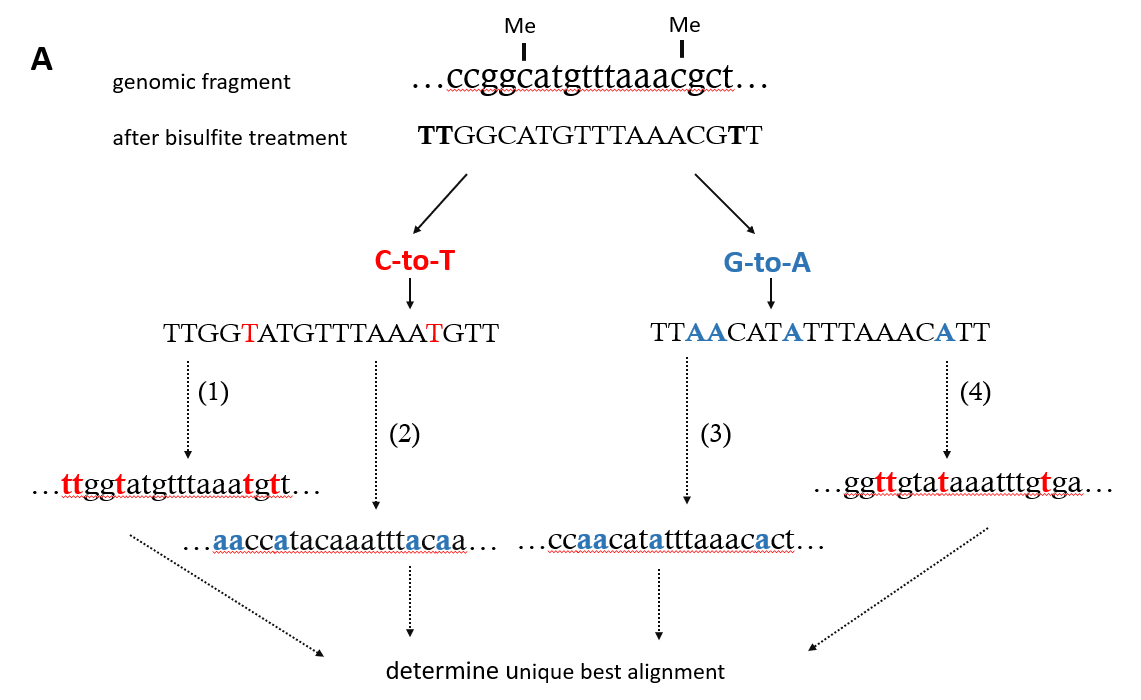
\includegraphics[scale=0.8]{figures/bismark-a.png}
  \caption{\textbf{Bismark’s approach to bisulfite mapping.}
  The bisulfite-treated reads were converted to C-to-T and G-to-A versions and then aligned with the reference genome equivalent conversion. These four reads are aligned in parallel to produce the unique best alignment.}
  \label{f3}
\end{figure}

\begin{figure}[h!]
  \centering
  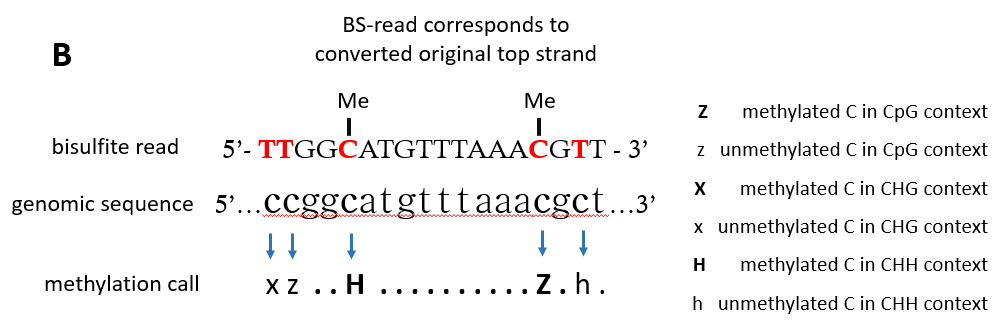
\includegraphics[scale=0.8]{figures/bismark-b.png}
  \caption{\textbf{A diagram of the three methylation situations shown in Bismark.}
  The capital and small letters of Z, X, and H were used to distinguish between different cases of cytosine and whether methylation had occurred.}
  \label{f4}
\end{figure}


Third, to remove from the mapped output file the alignments at the same position of the genome, use "deduplicate" to remove duplicate aligned reads. This situation may be caused by excessive PCR amplification, but this step is only appropriate for WGBS, not for RRBS, amplicon, or other target enrichment-type libraries!

Finally, to enable methylation analysis in different sequence contexts and model organisms, the methylation calling in Bismark considers the surrounding sequences (CpG, CHG, and CHH). Each cytosine position is written to a new output file, with "+" indicating a methylated cytosine and "-" indicating a non-methylated cytosine. The output of the methylation will distinguish between three methylation states, CpG, CHG, or CHH, and can be obtained in either a combined or aligned chain-specific format. In addition, the output can be converted to other formats such as SAM/BAM, or imported into genome browsers such as SeqMonk to visualize the results of its mapping.

\section{Bowtie2}
Bowtie is a common software for sequence alignment and sequence analysis in biology, and Bowtie2 introduced here is a fast and memory-saving tool used to align sequencing reads with reference sequences\cite{langmead2012fast}. It is especially good at aligning longer genomes, such as mammalian genomes, with reads of approximately 50 to 1000 bp in length. Since Bowtie2 uses FM indexes to build indexes on genomes, the indexes occupy a memory space. Bowtie2 supports gapped, local, and paired-end alignment modes. In addition, it can utilize multiple processors in parallel to accelerate alignment performance.

Bowtie2 outputs the alignment in SAM format so that we can use SAM files to process other tools such as SAMtools, GATK, etc.  Bowtie2 is also frequently used in genomics, including for variant calling, BS-seq, RNA-seq, CHIP-seq, and differential gene expression. Compared with Bowtie 1, Bowtie 2 has the following advantages:\\
(1) For reads longer than 50bp, Bowtie2 is more accurate and faster while using less memory space; however, for reads smaller than 50bp, Bowtie1 is often faster and more accurate.\\
(2) Bowtie2 supports gapped alignment with affine gap penalties. The number of gaps and gap lengths are not restricted.Bowtie 1 finds just ungapped alignments.\\
(3) Bowtie2 supports local alignment and end-to-end alignment (Figure \ref{f5}). Bowtie1 requires reads to be perfectly aligned.\\
(4) Bowtie2 does not limit the length of reads; while Bowtie1 reads the maximum length of about 1000bp.\\
(5) Bowtie2 allows “N” in the reference sequence, while Bowtie1 does not support it.\\

\begin{figure}[h]
  \centering
  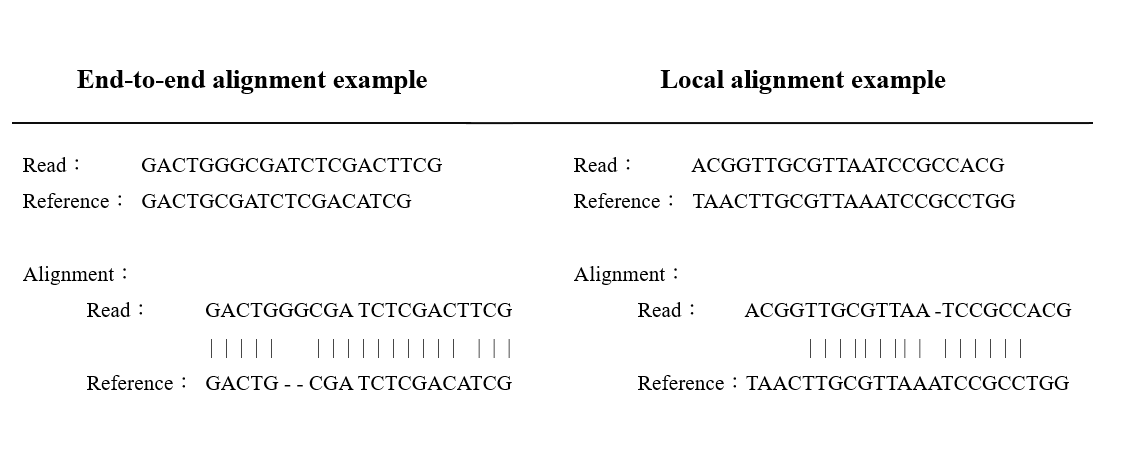
\includegraphics[scale=0.8]{figures/bowtie2_align.png}
  \caption{\textbf{End-to-end alignment versus local alignment.}
  }
  \label{f5}
\end{figure}

(Figure \ref{f5})Where dash symbols represent gaps and vertical bars show where aligned characters match.(1)End-to-end alignment:“end-to-end” alignment involves all the characters in the read.Such an alignment can be produced by Bowtie 2 in either end-to-end mode or in local mode.(2)Local alignment:local alignment does not participate in some characters at the end of reads. In this case, 4 characters are omitted (or "soft trimmed" or "soft clipped") from the beginning and 3 characters are omitted from the end. This sort of alignment can be produced by Bowtie 2 only in local mode.

When we actually perform the alignment sequence step, it often takes a lot of time in the step. This is because the aligner has to deal with difficult computational problems and must determine the possible starting points of the reads relative to the reference genome for each read. Therefore, we have to reduce the difficulty of this step by using index and dynamic programming. Therefore, most of the alignment software is divided into two commands: index creation and actual alignment.

\chapter{Experiment and Results}
\section{Dataset}
In section 3.1, we will introduce the data used in the experiment, which can be divided into two parts: the actual data and the simulated data. Since there are not many benchmark data available, we will use the tool MethylFASTQ to simulate the occurrence of methylation and assist us in the analysis of the alignment tool. With the data generated from the simulation tool, we can easily know the methylation situation of each site, which is very helpful for us to evaluate the accuracy of the alignment tool.

\subsection{Bisulfite sequencing real data}
The real data come from the WGBS library of Arabidopsis thaliana available from NCBI. Arabidopsis thaliana is a common model organism in plant biology and genetics, with a relatively small genome of about 135 million base pairs. We used TAIR10 chromosome files as the reference genome for this experiment and selected the Illumina-sequenced Bisulfite-seq SRR5534888 as the read. a sample of GSM2616974 was used as the gold standard for our methylation analysis to help us evaluate the accuracy of different tools later. The methylation level is an important criterion for the evaluation of our tools, which is calculated by the number of methylated cytosines (C) divided by the total number of cytosines. For the data with bisulfite sequencing, the total number of cytosines in the total number of cytosines and thymines in the read. In the following experiments of real data, we chose BS-Seeker2 and Bismark as the bisulfite alignment tools for the analysis.

\subsection{Generating simulation data using MethylFASTQ}
In this paper, we used MethylFASTQ as a simulator to generate experimental data. For the reference genome section, we chose two different species, namely chromosome 22 of GRCh37 in the human genome library and chromosome M in Arabidopsis thaliana. Chromosome 22 is one of the 23 pairs of chromosomes in human cells, and in normal human cells, there is usually one pair of chromosome 22. Moreover, chromosome 22 is the first human chromosome to be completely sequenced. In the following experiments, we will capture the target fragments to analyze different bisulfite alignment tools.


% \begin{table}
% \begin{tabularx}{0.9\linewidth}{lX}
% Notation                                               &  Description\\
% \toprule
% $P_{\text{meth}\,|\,\textsf{context,BG}}$                    &  The background probability of methylation by context.\\[.3ex]
% $n_{\textsf{context},\,i}$                                 &  The number of cytosines (with sufficient read coverage)\newline of the given context occurring at position $i$ in the set of TFBS.\\[.3ex]
% $\overline{v}\,|\,\scriptstyle{\textsf{context},i}$  & The average methylation values of those cytosines.\\
% \bottomrule
% \end{tabularx}
% \caption{Summary of notation used in this thesis.}
% \label{tab:notation}
% \end{table}

\section{BS-Seeker2 and Bismark}
\subsection{Experimental results of BS-Seeker2}
First, BS-Seeker2 would filter the reads and filter out the low-quality reads, and then help us to get the unique reads before mapping. but this function is only for WGBS, not for RRBS. Next, build the index for the reference genes, and the reference genome if it is RRBS, then we need to give the fragment lengths of upper and lower bounds. After doing the previous two steps, we perform the alignment of the read with the reference genome sequence. This step is also the most time-consuming part of BS-Seeker2, which took more than 11 hours to complete. The experimental results showed that the total number of sequences was 169,961,140 and the number of uniquely mapped reads accounted for 10,379,352,749, with a mapping rate of about 80.22\%.

Finally, calls methylation levels from the mapping result, this step can be split into three parts: (i) sorting BS-Seeker2 alignments; (ii) indexing sorted alignment; (iii) calculating methylation levels. After the above steps, a total of three output files will be produced, wig file, CGmap file, and ATCGmap file. (Figure \ref{f6}) is one of the BS-Seeker2 output files, CGmap files, which contains the following information including: chromosome, nucleotide on Watson (+) strand, position, context (CG/CHG/CHH), methylation-level, etc.

\begin{figure}[h]
  \centering
  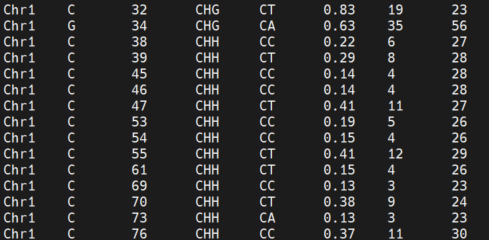
\includegraphics[scale=0.8]{table/CGmap.png}
  \caption{\textbf{The output files of BS-Seeker2.}
  }
  \label{f6}
\end{figure}


\subsection{Experimental results of Bismark}
(Figure \ref{f7}) shows the alignment information after preprocessing and running Bismark. The first row shows the total number of sequences used for analysis, with 169,961,140 sequences, and the second row shows the unique hits reads, with 118,548,486 sequences. Compared with the BS-Seeker2, there are less than 21,446,287 reads in this part.

\begin{figure}[h]
  \centering
  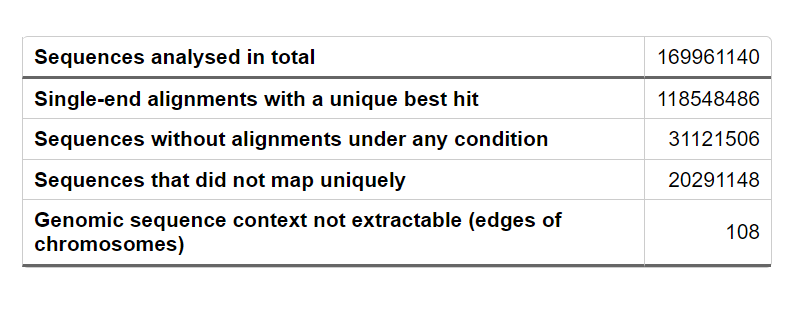
\includegraphics[scale=0.8]{table/table_alignment_Stats.png}
  \caption{\textbf{Alignment Stats.}
  }
  \label{f7}
\end{figure}

(Figure \ref{f8})shows the distribution of different alignments in Bismark, where unique alignments are about 69.8\% , multiple alignments are about 11.9\%, and mappability is about 81.7\%, which has similar results with BS-Seeker2.

\begin{figure}[h]
  \centering
  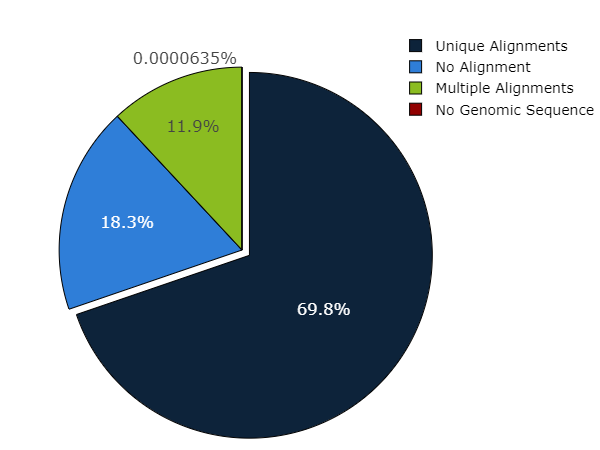
\includegraphics[scale=0.4]{figures/align_fig.png}
  \caption{\textbf{Alignment Stats.}
  }
  \label{f8}
\end{figure}

(Figure \ref{f9}) shows the percentages of the three methylation states before and after the deduplication step, and the deduplication step will remove the repeated reads. At the same time, it also reduces the computation time spent on repeated reads and further optimizes the results of the experiment.

\begin{figure}[h]
  \centering
  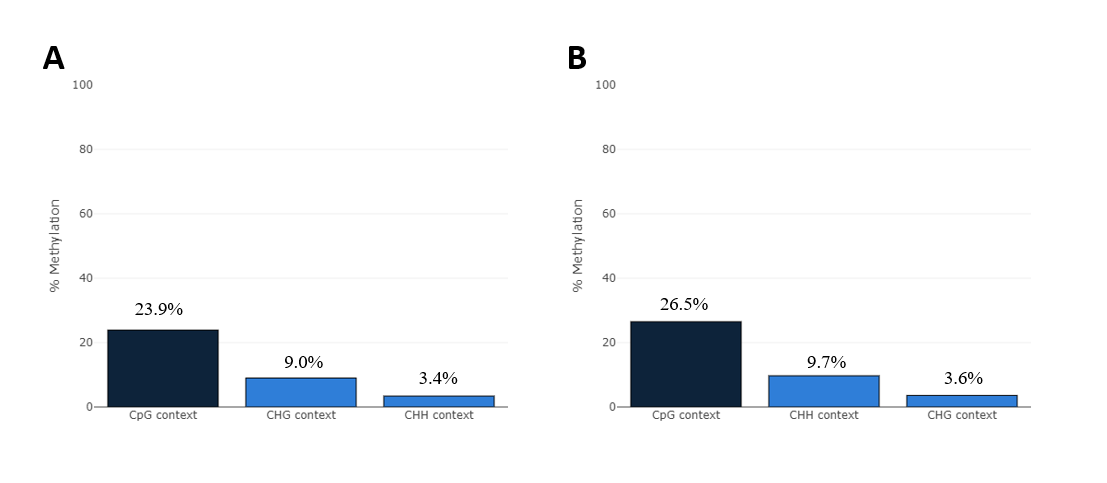
\includegraphics[scale=0.8]{figures/cytosine_methylation.png}
  \caption{\textbf{Cytosine methylation.}
  }
  \label{f9}
\end{figure}

Figure (A) shows the percentage of methylation generated before deduplication; Figure (B) shows the percentage of methylation generated after deduplication.

\subsection{Compare the results of BS-Seeker2 and Bismark}
In this chapter, we use real data to perform experiments with Arabidopsis thaliana, and we can get some helpful information from the experimental results of BS-Seeker2 and Bismark. First, we can get the individual percentages of the two tools in the three methylation states, except for the methylation difference on CpG which is more obvious (1.82\% difference), the percentages of methylation in the other two states are very similar (Figure \ref{f10}). Second, we divided the results into seven chromosomes to discuss, calculated the average methylation level of each chromosome respectively, and compared them with our benchmark (Figure \ref{f11}). We first observe the average methylation level of all chromosomes, the average methylation level of BS-Seeker2 is 0.1991, the average methylation level of Bismark is 0.2263, and the average methylation level of Benchmark is 0.2219. We can find from the average methylation level between different tools that in the case of real data Bismark and Benchmark have similar methylation levels.

\begin{figure}[h]
  \centering
  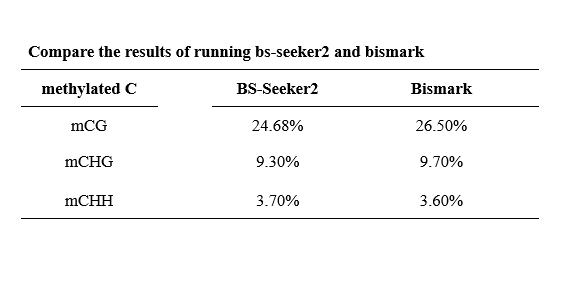
\includegraphics[scale=0.8]{table/table3.png}
  \caption{\textbf{Compare the results of running BS-seeker2 and Bismark.}
  }
  \label{f10}
\end{figure}

\begin{figure}[h]
  \centering
  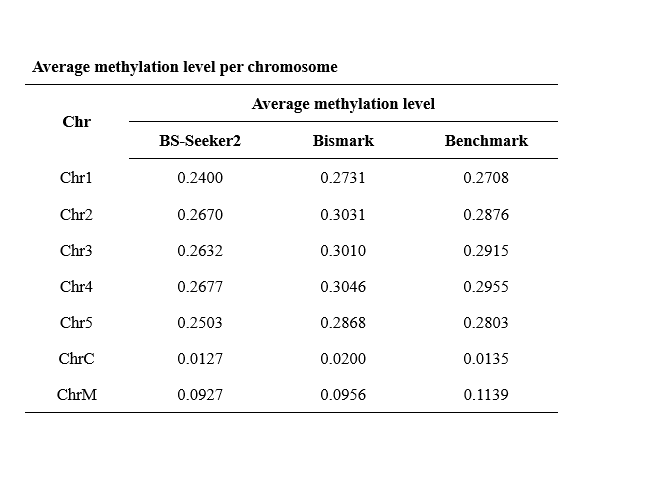
\includegraphics[scale=0.8]{table/table4.png}
  \caption{\textbf{Average methylation level per chromosome.}}
  \label{f11}
\end{figure}

Third, we calculate the deviation value of each site in the chromosome and benchmark and use the deviation value to determine the accuracy of methylation evaluation between different tools. First, we will use the result files obtained from bisulfite mapping tools and compare the sites in tools with those in the benchmark. If both files have the same sites, we will subtract the methylation level of tools from the methylation level of the benchmark and take the absolute value.Because we only care about the difference between the tool and the benchmark, we do not need to consider the case of positive and negative signs. Then, the deviation values just calculated were summed and averaged to be the criterion for our evaluation of the accuracy of the tool. (Figure \ref{f12}) shows the deviation values between BS-Seeker2 and Bismark and the benchmark. The lower the deviation value, the closer the predicted methylation level of the tool is to the standard answer, while the higher the deviation value, the greater the difference between the methylation level of the tool and the standard answer.

\begin{figure}[h]
  \centering
  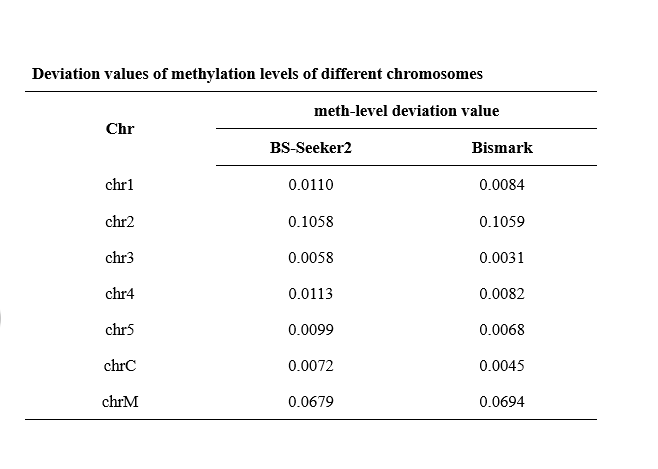
\includegraphics[scale=0.8]{table/table5.png}
  \caption{\textbf{Deviation values of methylation levels of different chromosomes.}
  }
  \label{f12}
\end{figure}


\section{Simulated data analysis}
In the simulated data of humans and Arabidopsis thaliana, we used three tools, EAGLE-meth, BS-Seeker2, and Bismark, to further evaluate the accuracy of different tools for calculating methylation levels. (Figure \ref{f13}) shows the functional descriptions of the three tools supported by the comparison.

\begin{figure}[h]
  \centering
  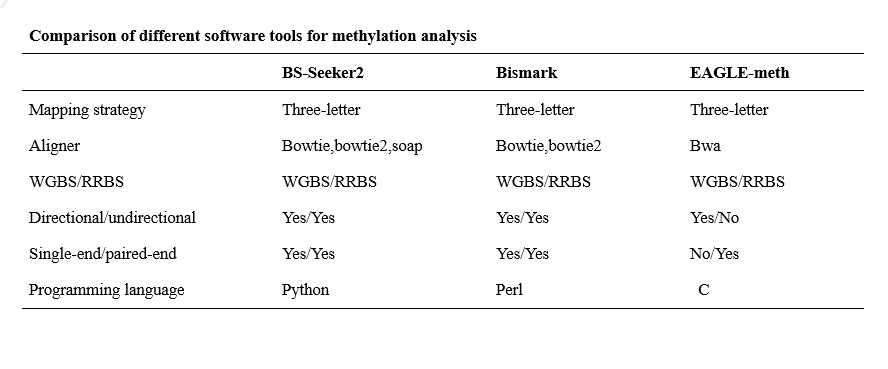
\includegraphics[scale=0.8]{table/table6.png}
  \caption{\textbf{Comparison of different software tools for methylation analysis.}}
  \label{f13}
\end{figure}

In setting the parameters of the simulation tool, we set the --cg CG-methylation-probability to " 0.3", which means that the average methylation rate of cytosine in the CG context is 30\%. Since CpG is the most common methylation scenario in mammals, we only considered methylation in the CpG context in the simulation data and set the methylation probability to “0” for both CHG and CHH. (Figure \ref{f14}) shows the results of the three bisulfite alignment tools, the average methylation level between the tools, and the deviation between the results of the tools and benchmark answers calculated. The “MCF” represents the positive “methylation calling file” generated after running MethylFASTQ. The “Average meth-level” refers to the average methylation level of each chromosome, and the “Meth-level deviation value” refers to the deviation value of the methylation level of each site and benchmark. The smaller the deviation value is, the closer the methylation level of the tool is to the benchmark.

\begin{figure}[h]
  \centering
  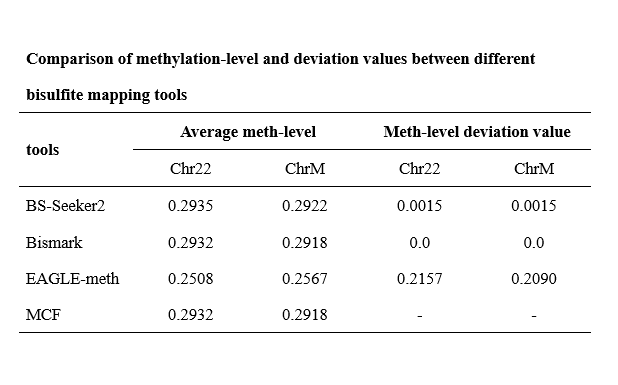
\includegraphics[scale=0.8]{table/table7.png}
  \caption{\textbf{Comparison of methylation-level and deviation values between different bisulfite mapping tools.}}
  \label{f14}
\end{figure}


\chapter{Conclusions and Future Work}

\section{Conclusions}
The experimental results are based on the simulated data of different species, we consider EAGLE-meth as a comparative tool for evaluating the bisulfite data. Using the experimental methylation probabilities and calculating the deviations between EAGLE-meth and benchmark, we can observe that the deviations are not high and are similar to the benchmark results. Therefore, EAGLE-meth has been able to estimate the methylation probability of most CpGs, which is a great help to the study of DNA methylation.

\section{Future Work}
Finally, we found that there are still some noteworthy problems. In the simulated data, we only choose the fragment of chr22 and chrM for the experiment. This is because the reference genome is a very long sequence, and EAGLE-meth adopts a greedy algorithm strategy, which will spend a lot of time in the actual computation. In addition, EAGLE-meth cannot be applied to longer genomic sequences because of memory limitations.


% \chapter{Discussion}
% Discussion the significance or your results.

% \chapter{Conclusion}
% Add your conclusions here.


\newpage
\AddToContents{Bibliography}
\printbibliography


\end{document}
